\fancyhead[LE]{\fontsize{8.5pt}{10pt}\selectfont\textbf{\textsf{\thepage}}\quad \textbf{\textsf{CHƯƠNG 1}}\quad \textsf{Các hàm số và Mô hình}}
\fancyhead[RO]{\fontsize{8.5pt}{10pt}\selectfont\textsf{MỤC 1.3}\quad \textsf{Hàm mới từ các hàm cũ}\quad \textbf{\textsf{\thepage}}}

\noindent
\begin{minipage}[t]{0.265\textwidth}
    \fontsize{8pt}{10pt}\selectfont
    \vspace*{155pt}
    \begin{center}
        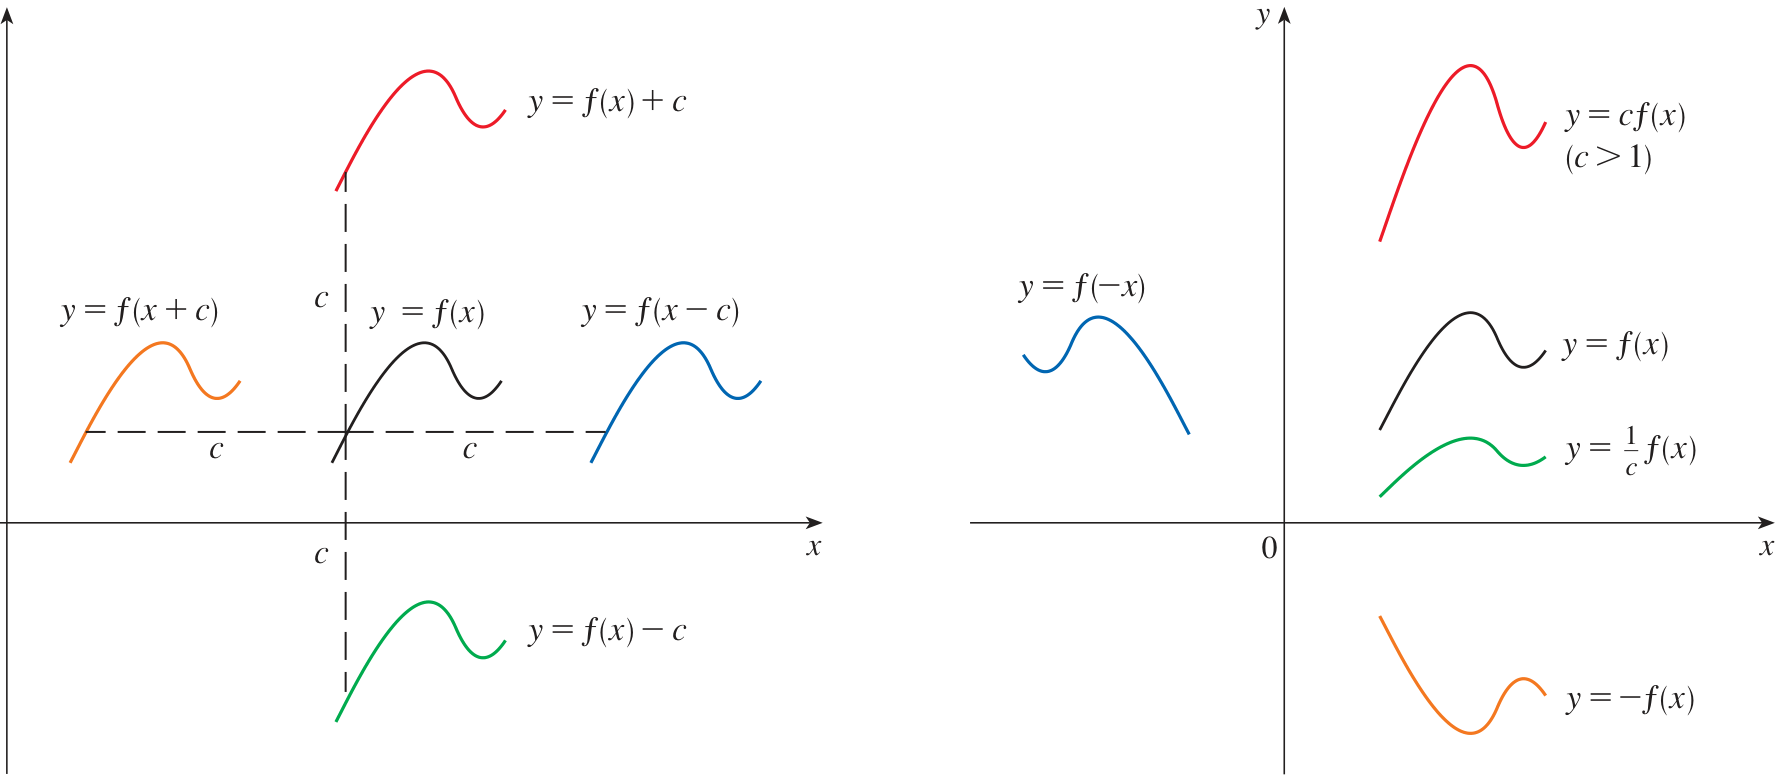
\includegraphics[width=0.92\linewidth]{images/p0072_fig1.png}\\[4pt]
        {\fontsize{7.5pt}{9.5pt}\selectfont\textbf{\textsf{HÌNH 1}}\quad \textsf{Tịnh tiến đồ thị của $f$}}
    \end{center}
\end{minipage}%
\hfill
\begin{minipage}[t]{0.708\textwidth}
    \fontsize{9.3pt}{13.2pt}\selectfont
    Trước hết, hãy xem xét **phép tịnh tiến** của đồ thị. Nếu $c$ là một số dương, thì đồ thị của $y = f(x) + c$ chính là đồ thị của $y = f(x)$ được tịnh tiến lên trên một khoảng bằng $c$ đơn vị (vì mỗi tung độ $y$ đều tăng thêm cùng một số $c$). Tương tự, nếu $g(x) = f(x - c)$, với $c > 0$, thì giá trị của $g$ tại $x$ bằng với giá trị của $f$ tại $x - c$ (nằm cách $x$ một khoảng $c$ đơn vị về phía bên trái). Do đó, đồ thị của $y = f(x - c)$ chính là đồ thị của $y = f(x)$ được tịnh tiến sang phải một khoảng $c$ đơn vị (xem Hình~1).

    \begin{definitionbox}
        \textbf{\textsf{\color{stewartred}Phép tịnh tiến theo phương đứng và phương ngang}}\quad Giả sử $c > 0$. Để nhận được đồ thị của:
        \vspace{4pt}

        \noindent
        \begin{tabular}{@{}ll@{}}
        $y = f(x) + c$, & tịnh tiến đồ thị của $y = f(x)$ lên trên một khoảng $c$ đơn vị \\
        $y = f(x) - c$, & tịnh tiến đồ thị của $y = f(x)$ xuống dưới một khoảng $c$ đơn vị \\
        $y = f(x - c)$, & tịnh tiến đồ thị của $y = f(x)$ sang phải một khoảng $c$ đơn vị \\
        $y = f(x + c)$, & tịnh tiến đồ thị của $y = f(x)$ sang trái một khoảng $c$ đơn vị
        \end{tabular}
    \end{definitionbox}

    \begin{center}
    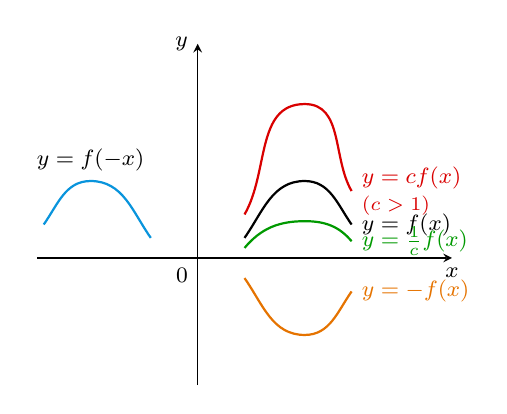
\begin{tikzpicture}[scale=0.85, >=stealth, baseline=(current bounding box.center)]
        % Trục tọa độ
        \draw[->] (-2.4,0) -- (3.8,0) node[below] {\footnotesize $x$};
        \draw[->] (0,-1.9) -- (0,3.2) node[left] {\footnotesize $y$};
        \node[below left] at (0,0) {\footnotesize $0$};

        % y = f(x) (đường gốc, màu đen)
        \draw[thick] (0.7,0.3) to[out=55, in=180] (1.6,1.15) to[out=0, in=125] (2.3,0.5) node[right] {\footnotesize $y = f(x)$};

        % y = cf(x) (c > 1, màu đỏ)
        \draw[thick, red!85!black] (0.7,0.65) to[out=60, in=180] (1.6,2.3) to[out=0, in=120] (2.3,1.0) node[right, align=left] {\footnotesize $y = cf(x)$\\[-2pt]\scriptsize $(c > 1)$};

        % y = 1/c f(x) (màu xanh lá)
        \draw[thick, green!60!black] (0.7,0.15) to[out=50, in=180] (1.6,0.55) to[out=0, in=130] (2.3,0.25) node[right] {\footnotesize $y = \frac{1}{c}f(x)$};

        % y = -f(x) (màu cam)
        \draw[thick, orange!90!black] (0.7,-0.3) to[out=-55, in=180] (1.6,-1.15) to[out=0, in=-125] (2.3,-0.5) node[right] {\footnotesize $y = -f(x)$};

        % y = f(-x) (màu lam)
        \draw[thick, cyan!80!blue] (-0.7,0.3) to[out=125, in=0] (-1.6,1.15) to[out=180, in=55] (-2.3,0.5);
        \node[above] at (-1.6,1.15) {\footnotesize $y = f(-x)$};
    \end{tikzpicture}\\[4pt]
    {\fontsize{8.5pt}{10.5pt}\selectfont\textbf{\textsf{HÌNH 2}}\quad \textsf{Co giãn và phản xạ đồ thị của $f$}}
    \end{center}

    Bây giờ, hãy xem xét các phép biến đổi **co giãn** và **phản xạ (đối xứng)**. Nếu $c > 1$, thì đồ thị của $y = cf(x)$ là đồ thị của $y = f(x)$ được giãn theo phương đứng theo hệ số $c$ (vì mỗi tung độ $y$ đều được nhân với cùng một số $c$). Đồ thị của $y = -f(x)$ là đồ thị của $y = f(x)$ lấy đối xứng qua trục $x$ do điểm $(x, y)$ được thay thế bởi điểm $(x, -y)$. (Xem Hình~2 và bảng tóm tắt sau đây, trong đó cũng nêu kết quả của các phép co, giãn và phản xạ khác.)

    \begin{definitionbox}
        \textbf{\textsf{\color{stewartred}Phép co giãn và phản xạ theo phương đứng và phương ngang}}\quad Giả sử $c > 1$. Để nhận được đồ thị của:
        \vspace{4pt}

        \noindent
        \begin{tabular}{@{}ll@{}}
        $y = cf(x)$, & giãn đồ thị của $y = f(x)$ theo phương đứng theo hệ số $c$ \\
        $y = (1/c)f(x)$, & co đồ thị của $y = f(x)$ theo phương đứng theo hệ số $c$ \\
        $y = f(cx)$, & co đồ thị của $y = f(x)$ theo phương ngang theo hệ số $c$ \\
        $y = f(x/c)$, & giãn đồ thị của $y = f(x)$ theo phương ngang theo hệ số $c$ \\
        $y = -f(x)$, & lấy phản xạ đồ thị của $y = f(x)$ qua trục $x$ \\
        $y = f(-x)$, & lấy phản xạ đồ thị của $y = f(x)$ qua trục $y$
        \end{tabular}
    \end{definitionbox}
\end{minipage}